\documentclass[10pt]{beamer}
\usetheme{jambro}

\title[]{Macroeconomia I - Modelo clássico}
\author[]{Paulo Victor da Fonseca}
\date{09 de março de 2023}

\hypersetup{
    colorlinks = true,
    urlcolor = teal,
    linkcolor = teal    
}
\usepackage[portuguese]{babel}
\usepackage{subfig}
\usepackage{emoji}

\begin{document}

\begin{frame}[plain]
    \titlepage{
        \begin{center}
            \begin{minipage}{0.8\textwidth}
                \centering
            \end{minipage}
        \end{center}}
\end{frame}

\begin{frame}{Sumário}
    \tableofcontents
\end{frame}

\section{Lei de Say}
\begin{frame}
    {Lei de Say}
    \begin{itemize}
        \item \hlight{Lei de Say}: ``a oferta cria sua própria demanda'' \bigskip
        \item Como o ato de produção de bens e serviços cria, simultaneamente, renda e poder de compra, não haveria impedimento ao pleno emprego causado por deficiência de demanda agregada\bigskip
        \item A lei, no entanto, não nega a possibilidade de ocorrência de uma má-alocação de recursos e que uma superprodução de certos bens possa acontecer\bigskip
        \item Entretanto, esse problema seria apenas temporário e um excesso de oferta não é possível ao considerarmos o conjunto de todos os bens (superprodução generalizada) 
    \end{itemize}
\end{frame}

\begin{frame}
    {Lei de Say}
    \begin{itemize}
        \item Lei de Say - enunciada originalmente para um contexto de economia de escambo (por definição, o ato de ofertar um bem implica, necessariamente, uma demanda por outro bem)\bigskip
        \item De maneira geral, economistas clássicos (Ricardo e Mill) sustentaram a lei de Say e acreditavam ser válida, também, para economia de trocas com moeda\bigskip
        \item Para eles, a moeda nada mais é que um meio de troca conveniente que possibilita aos participantes do mercado evitarem as inconveniências de um sistema de escambo\bigskip
        \item Se a lei de Say é válida para uma economia com moeda, então, um mercado é garantido para qualquer nível de produto que for produzido, mesmo que as forças de mercado levem a mudanças na composição do produto agregado\bigskip
        \item Se demanda agregada e oferta agregada sempre se equalizam, a \hlight{moeda nada mais é que um ``véu'' cobrindo as forças reais subjacentes de uma economia}
    \end{itemize}
\end{frame}

\begin{frame}
    {Lei de Say}
    \begin{enumerate}
        \item \tikz[tstyle]{\node[nstyle](node0){Versão fraca da lei de Say}}: cada ato de produção e oferta envolve, necessariamente, a criação, de maneira geral, de uma demanda equivalente. \hlight{Mas nada assegura que a quantidade produzida seja consistente com equilíbrio de pleno emprego}. Qualquer nível de produto agregado que ocorra encontrará um mercado. Essa versão se aplica tanto a baixos níveis de produto agregado quanto a níveis elevados\bigskip        
        \item \tikz[tstyle]{\node[nstyle](node1){Versão forte da lei de Say}}: numa economia competitiva de mercado, haverá tendência automática ao estabelecimento do pleno emprego. Equivalente à proposição de que não há obstáculos ao pleno emprego em termos de deficiência de demanda agregada\bigskip
    \end{enumerate}
    \begin{itemize}
        \item Para ver como clássicos justificavam crença na versão forte da lei de Say, estudaremos as ideias que relacionam investimento, poupança e taxa real de juros
    \end{itemize}
    \begin{tikzpicture}[tpstyle]
        \draw[pencil,very thick, brick] ([yshift=-1pt]node0.south west) to ([yshift=-1pt]node0.south east);
        \draw[pencil,very thick, blue] ([yshift=-1pt]node1.south west) to ([yshift=-1pt]node1.south east);
    \end{tikzpicture}
\end{frame}

\section{Determinação da taxa de juros}
\begin{frame}
    {Teoria clássica de taxa de juros}
    \begin{itemize}
        \item \hlight{Teoria clássica de determinação da taxa de juros} - papel fundamental para assegurar que não ocorra deficiência de demanda agregada\bigskip
        \item Economia com dois setores - famílias e firmas - no equilíbrio, despesas agregadas ($E$) devem ser iguais ao produto agregado ($Y$)
        \begin{equation}
            E = C(r) + I(r) = Y
            \label{aula3_eq1}
        \end{equation}
        \item Despesa agregada: gastos com investimento ($I$) por parte das firmas + gastos com consumo ($C$) por parte das famílias\bigskip
        \item Modelo clássico: demanda pelos dois tipos de bens é função da taxa real de juros ($r$)
    \end{itemize}
\end{frame}

\begin{frame}
    {Teoria clássica de taxa de juros}
    \begin{itemize}
        \item Famílias não gastam automaticamente toda sua renda:
        \begin{equation}
            Y - C(r) = S(r)
            \label{aula3_eq2}
        \end{equation}
        \item Portanto:
        \begin{equation}
            S(r) = I(r)
            \label{aula3_eq3}
        \end{equation}
        \item Poupança ($S$) também é função da taxa de juros - quanto maior a taxa de juros, mais dispostos estarão os poupadores a substituir consumo presente por consumo futuro\bigskip
        \item \hlight{Taxa de juros como uma recompensa real pela ``abstinência'' ou parcimônia}
    \end{itemize}
\end{frame}

\begin{frame}
    {Teoria clássica de taxa de juros}
    \begin{itemize}
        \item Fluxo de poupança representa oferta de fundos emprestáveis no mercado de capitais\bigskip
        \item Como a poupança das famílias responde positivamente a variações na taxa de juros ($S'(r) > 0$), o consumo deve ser uma função negativamente relacionada à taxa de juros ($C'(r) < 0$)
    \end{itemize}
\end{frame}

\begin{frame}
    {Teoria clássica de taxa de juros}
    \begin{itemize}
        \item Gastos com investimento em bens de capital negativamente relacionados à taxa de juros ($I'(r)<0$) e representam demanda por fundos emprestáveis no mercado de capitais\bigskip
        \item Gastos com investimento só se justificam se a taxa de retorno esperada é maior (ou igual) ao custo de adquirir os fundos utilizados para a aquisição de bens de $K$\bigskip
        \item Quanto maior a taxa de juros, maiores os custos explícitos (e implícitos) dos fundos usados para aquisição de bens de $K$\bigskip
        \item Portanto, gastos das firmas com investimento ($I$) podem ser representados como função decrescente da taxa de juros ($r$)
    \end{itemize}
\end{frame}

\begin{frame}{Teoria clássica de taxa de juros}
    \begin{figure}
        \centering
        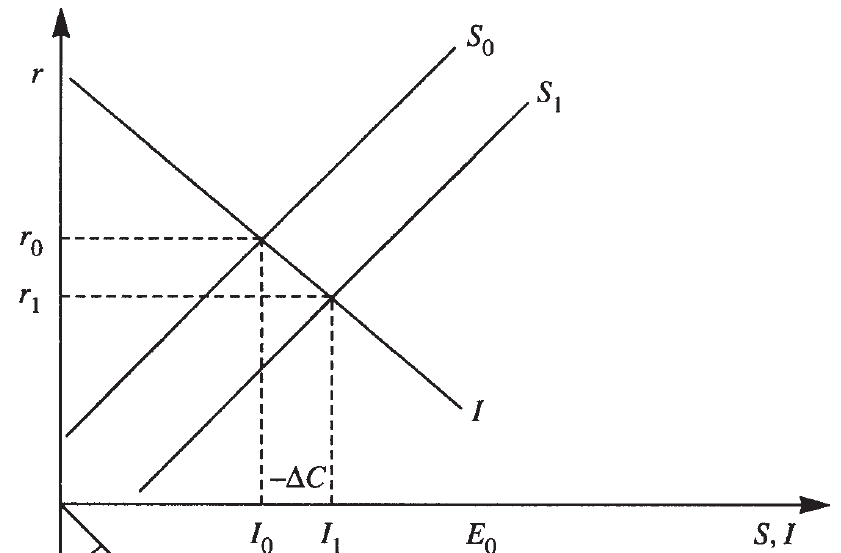
\includegraphics[width=0.65\textwidth]{./figures/aula3_fig1.PNG}
        \caption{Determinação da taxa de juros. Fonte: Snowdon e Vane (2005).}
        \label{aula3_fig1}
    \end{figure}
\end{frame}

\begin{frame}
    {Teoria clássica de taxa de juros}
    \begin{itemize}
        \item Na figura vemos como produtividade e parciônia determinam a taxa real de juros\bigskip
        \item Variações nas taxas de juros agem como uma força equilibradora que mantem a igualdade entre oferta e demanda de fundos emprestáveis, assegurando que demanda agregada nunca é deficiente
    \end{itemize}
\end{frame}

\section{Teoria clássica de taxa de juros e lei de Say}
\begin{frame}{Taxa de juros e lei de Say}
    \begin{figure}
        \centering
        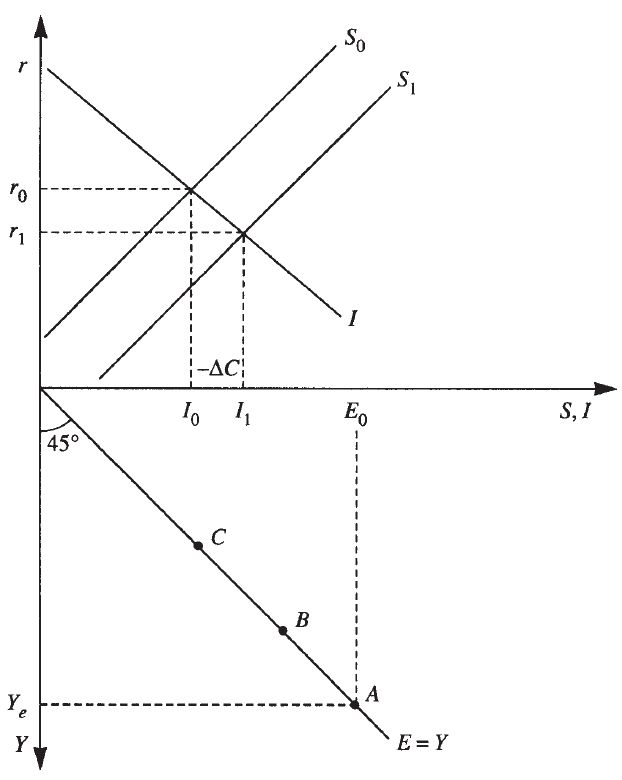
\includegraphics[width=0.35\textwidth]{./figures/aula3_fig2.PNG}
        \caption{Mecanismo clássico de taxa de juros e lei de Say. Fonte: Snowdon e Vane (2005).}
        \label{aula3_fig2}
    \end{figure}
\end{frame}

\begin{frame}
    {Taxa de juros e lei de Say}
    \begin{itemize}
        \item Na figura vemos a importância da flexibilidade da taxa de juros para o processo de equilíbrio clássico\bigskip
        \item Painel (a) - teoria clássica de determinação de taxa de juros\bigskip
        \item Painel (b) - igualdade entre produto agregado e demanda total por bens e serviços\bigskip
        \item Vimos que a competição no mercado de trabalho leva à emergência de um salário real e nível de emprego de equilíbrio que, combinados à função de produção, nos leva a um nível de produto compatível com o pleno emprego ($Y_e$)
    \end{itemize}
\end{frame}

\begin{frame}
    {Taxa de juros e lei de Say}
    \begin{itemize}
        \item Painel (b) - uma magnitude igual à $E_0$ de despesas agregadas é necessária para adquirir uma quantidade de produto agregado $Y_e$\bigskip
        \item Como oferta e demanda são iguais em todos os pontos ao longo da linha de $45º$, qualquer ponto é compatível com a versão fraca da lei de Say\bigskip
        \item O ponto $A$ corresponde à versão forte da lei de Say\bigskip
        \item Despesas e produto agregados em igualdade mas, além disso, $Y_e$ corresponde ao nível de produto agregado associado ao equilíbrio de pleno emprego no mercado de trabalho
    \end{itemize}
\end{frame}

\begin{frame}
    {Taxa de juros e lei de Say}
    \begin{itemize}
        \item Importância da flexibilidade de taxa de juros - o que aconteceria caso consumidores decidissem poupar mais (consumir menos)?\bigskip
        \item Curva de poupança desloca-se para a direita ($S_0$ para $S_1$ no painel (a))\bigskip
        \item Excesso de oferta inicial de fundos emprestáveis levaria a uma queda na taxa de juros de $r_0$ para $r_1$\bigskip
        \item Isso aumentaria atratividade dos bens de $K$ para firmas, aumentando gastos com investimento de $I_0$ para $I_1$\bigskip
        \item Como $E_0 - I_0$ é igual aos gastos com consumo das famílias, é evidente que o aumento com gastos de investimento, $I_1 - I_0$, compensa exatamente a queda nos gastos de consumo de $-\Delta C$\bigskip
        \item Portanto, \hlight{despesas agregadas permaneceriam em $E_0$, mas sua composição se altera}
    \end{itemize}
\end{frame}

\begin{frame}
    {Conclusões}
    \begin{itemize}
        \item Mesmo que decisões de poupar e investir sejam tomadas por diferentes agentes econômicos, a taxa de juros sofre alterações de maneira a conciliar desejos de poupar e investir\bigskip
        \item Na teoria Keynesiana, divergências entre poupança e investimento causam uma resposta quantitativa\bigskip
        \item No caso de um aumento de poupança, o modelo keynesiano prevê um declínio na despesa agregada, produto e emprego - \hlight{paradoxo da poupança}\bigskip
        \item No modelo clássico com lei de Say, flexibilidade de preços, salários e juros, pode apresentar mudanças na estrutura da demanda final, mas não permite deficiência de demanda prolongada e desemprego involuntário
    \end{itemize}
\end{frame}

\begin{frame}
    {Conclusões}
    \begin{itemize}
        \item Nem todos economistas aceitavam lei de Say e suas implicações\bigskip
        \item Malthus argumentava que um problema de superprodução generalizado de bens era possível\bigskip
        \item Ricardo e Mill - condições de oferta determinam produto agregado\bigskip
        \item Malthus (antecipando Keynes) - deu ênfase à demanda como fator determinante do produto agregado\bigskip
        \item Parte do ``conflito'' de visões entre Ricardo e Malthus tem origem no horizonte temporal adotado\bigskip
        \item Ricardo - preocupação com longo prazo. Malthus (e Keynes) - preocupação com curto prazo
    \end{itemize}
\end{frame}

\begin{frame}{Conclusões}
    \begin{tabular}{cl}
        \begin{tabular}{c}
            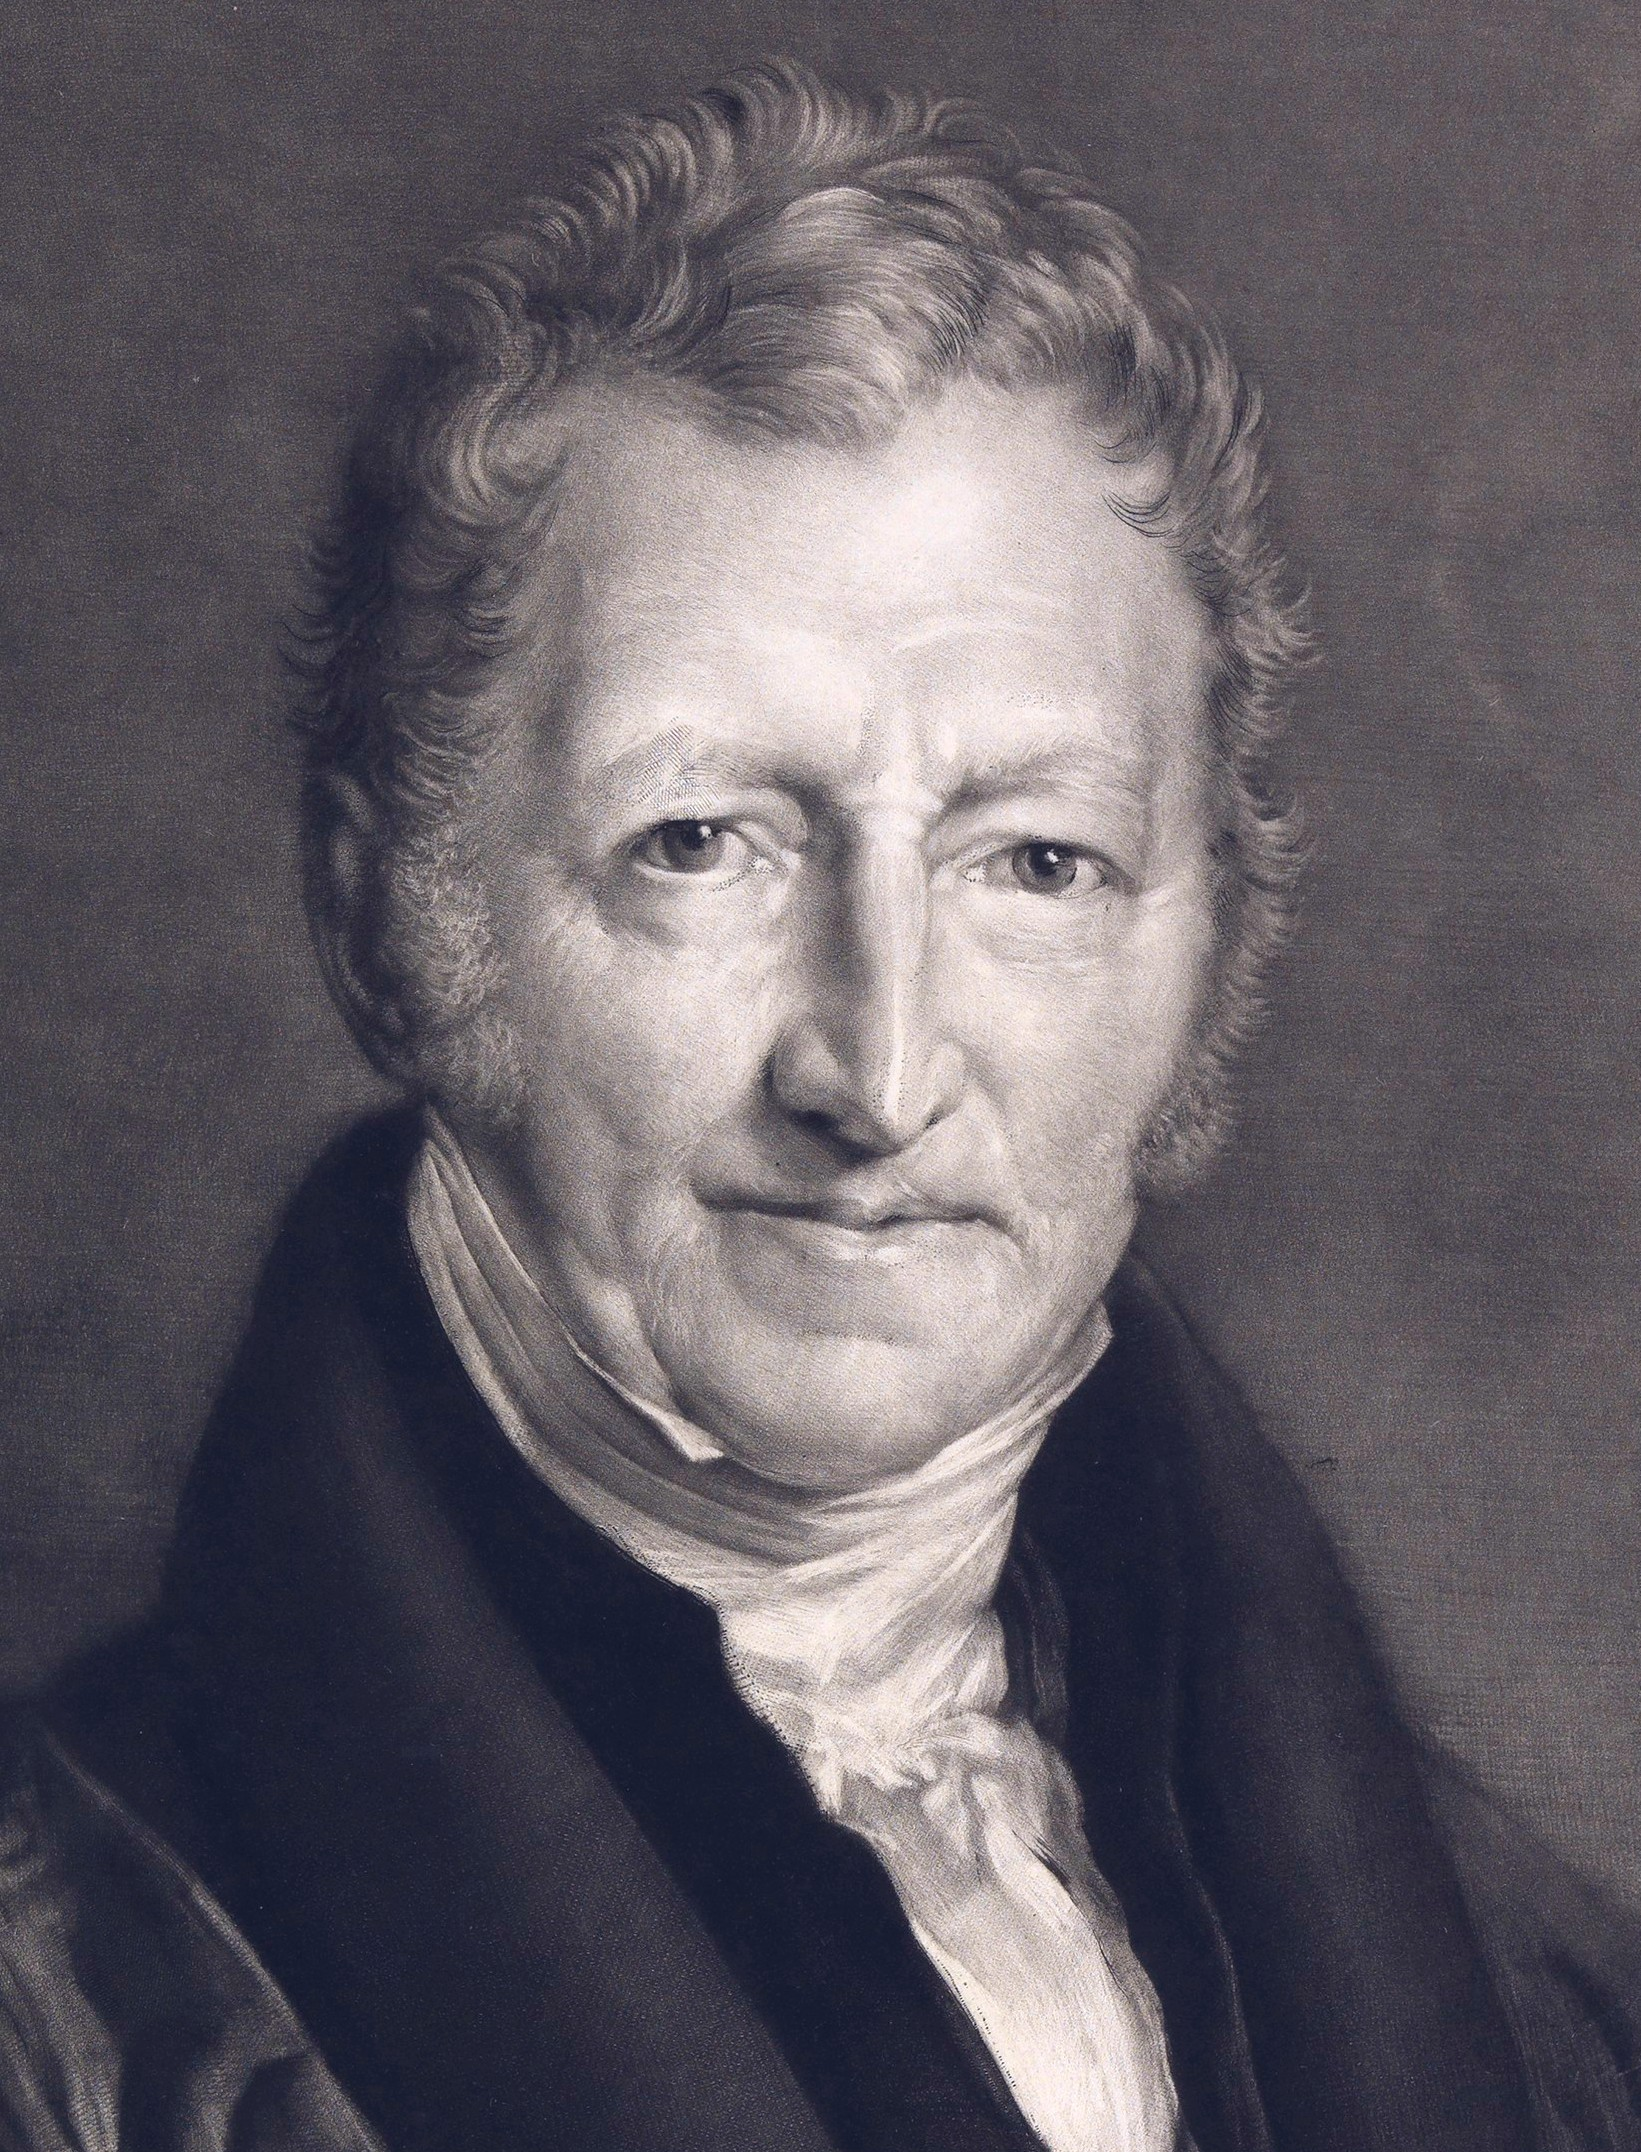
\includegraphics[width=3.5cm]{./figures/aula3_malthus.jpg} \\
            \tiny{{\scshape \href{https://pt.wikipedia.org/wiki/Thomas_Malthus}{Thomas Malthus (1766 - 1834)}}}
        \end{tabular}
         & \begin{tabular}{l}
               \parbox{0.6\linewidth}{%  change the parbox width as appropiate
                   \NB{"Ricardo conquistou a Inglaterra t\~{a}o completamente quanto a Santa Inquisi\c{c}\~{a}o conquistou a Espanha" \\ \begin{flushright} (Keynes, 1936)\end{flushright}}
               }
           \end{tabular} \\
    \end{tabular}
\end{frame}

\section{Teoria Quantitativa da Moeda}
\begin{frame}
    {Teoria quantitativa da moeda}
    \begin{itemize}
        \item Até agora focamos na determinação das variáveis reais\bigskip
        \item A operação dos mercados de trabalho e de capitais + lei de Say, possibilitou o desenvolvimento de um arcabouço teórico capaz de explicar as variáveis reais do sistema\bigskip
        \item Mas o que determina o nível de preços no modelo clássico?\bigskip
        \item \hlight{Teoria Quantitativa da Moeda}
    \end{itemize}
\end{frame}

\begin{frame}
    {Teoria quantitativa da moeda}
    \begin{itemize}
        \item Essência da macro clássica - separação entre variáveis reais e nominais\bigskip
        \item \hlight{Dicotomia clássica} possibilita examinar comportamento das variáveis reais ignorando as nominais\bigskip
        \item No sistema clássico que vimos até agora a quantidade de moeda em circulação é irrelevante para determinação das variáveis macro reais\bigskip
        \item \hlight{Neutralidade de longo prazo da moeda é uma propriedade crucial do modelo clássico}\bigskip
        \item Determinação das variáveis nominais no modelo clássico - \tikz[tstyle]{\node[nstyle](node0){Teoria Quantitativa da Moeda (TQM)}}
    \end{itemize}
    \begin{tikzpicture}[tpstyle]
        \draw[pencil,very thick, brick] ([yshift=-1pt]node0.south west) to ([yshift=-1pt]node0.south east);        
    \end{tikzpicture}    
\end{frame}

\begin{frame}{Teoria Quantitativa da Moeda}
    \begin{figure}
        \centering
        \subfloat[\href{https://pt.wikipedia.org/wiki/Richard_Cantillon}{Richard Cantillon ($\approx$ 1680 - 1734)}]{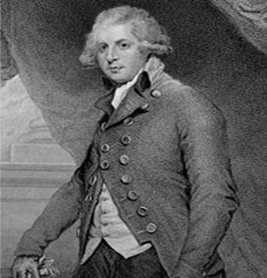
\includegraphics[width=0.3\textwidth]{./figures/aula3_cantillon.png}} \qquad
        \subfloat[\href{https://pt.wikipedia.org/wiki/David_Hume}{David Hume (1711 - 1776)}]{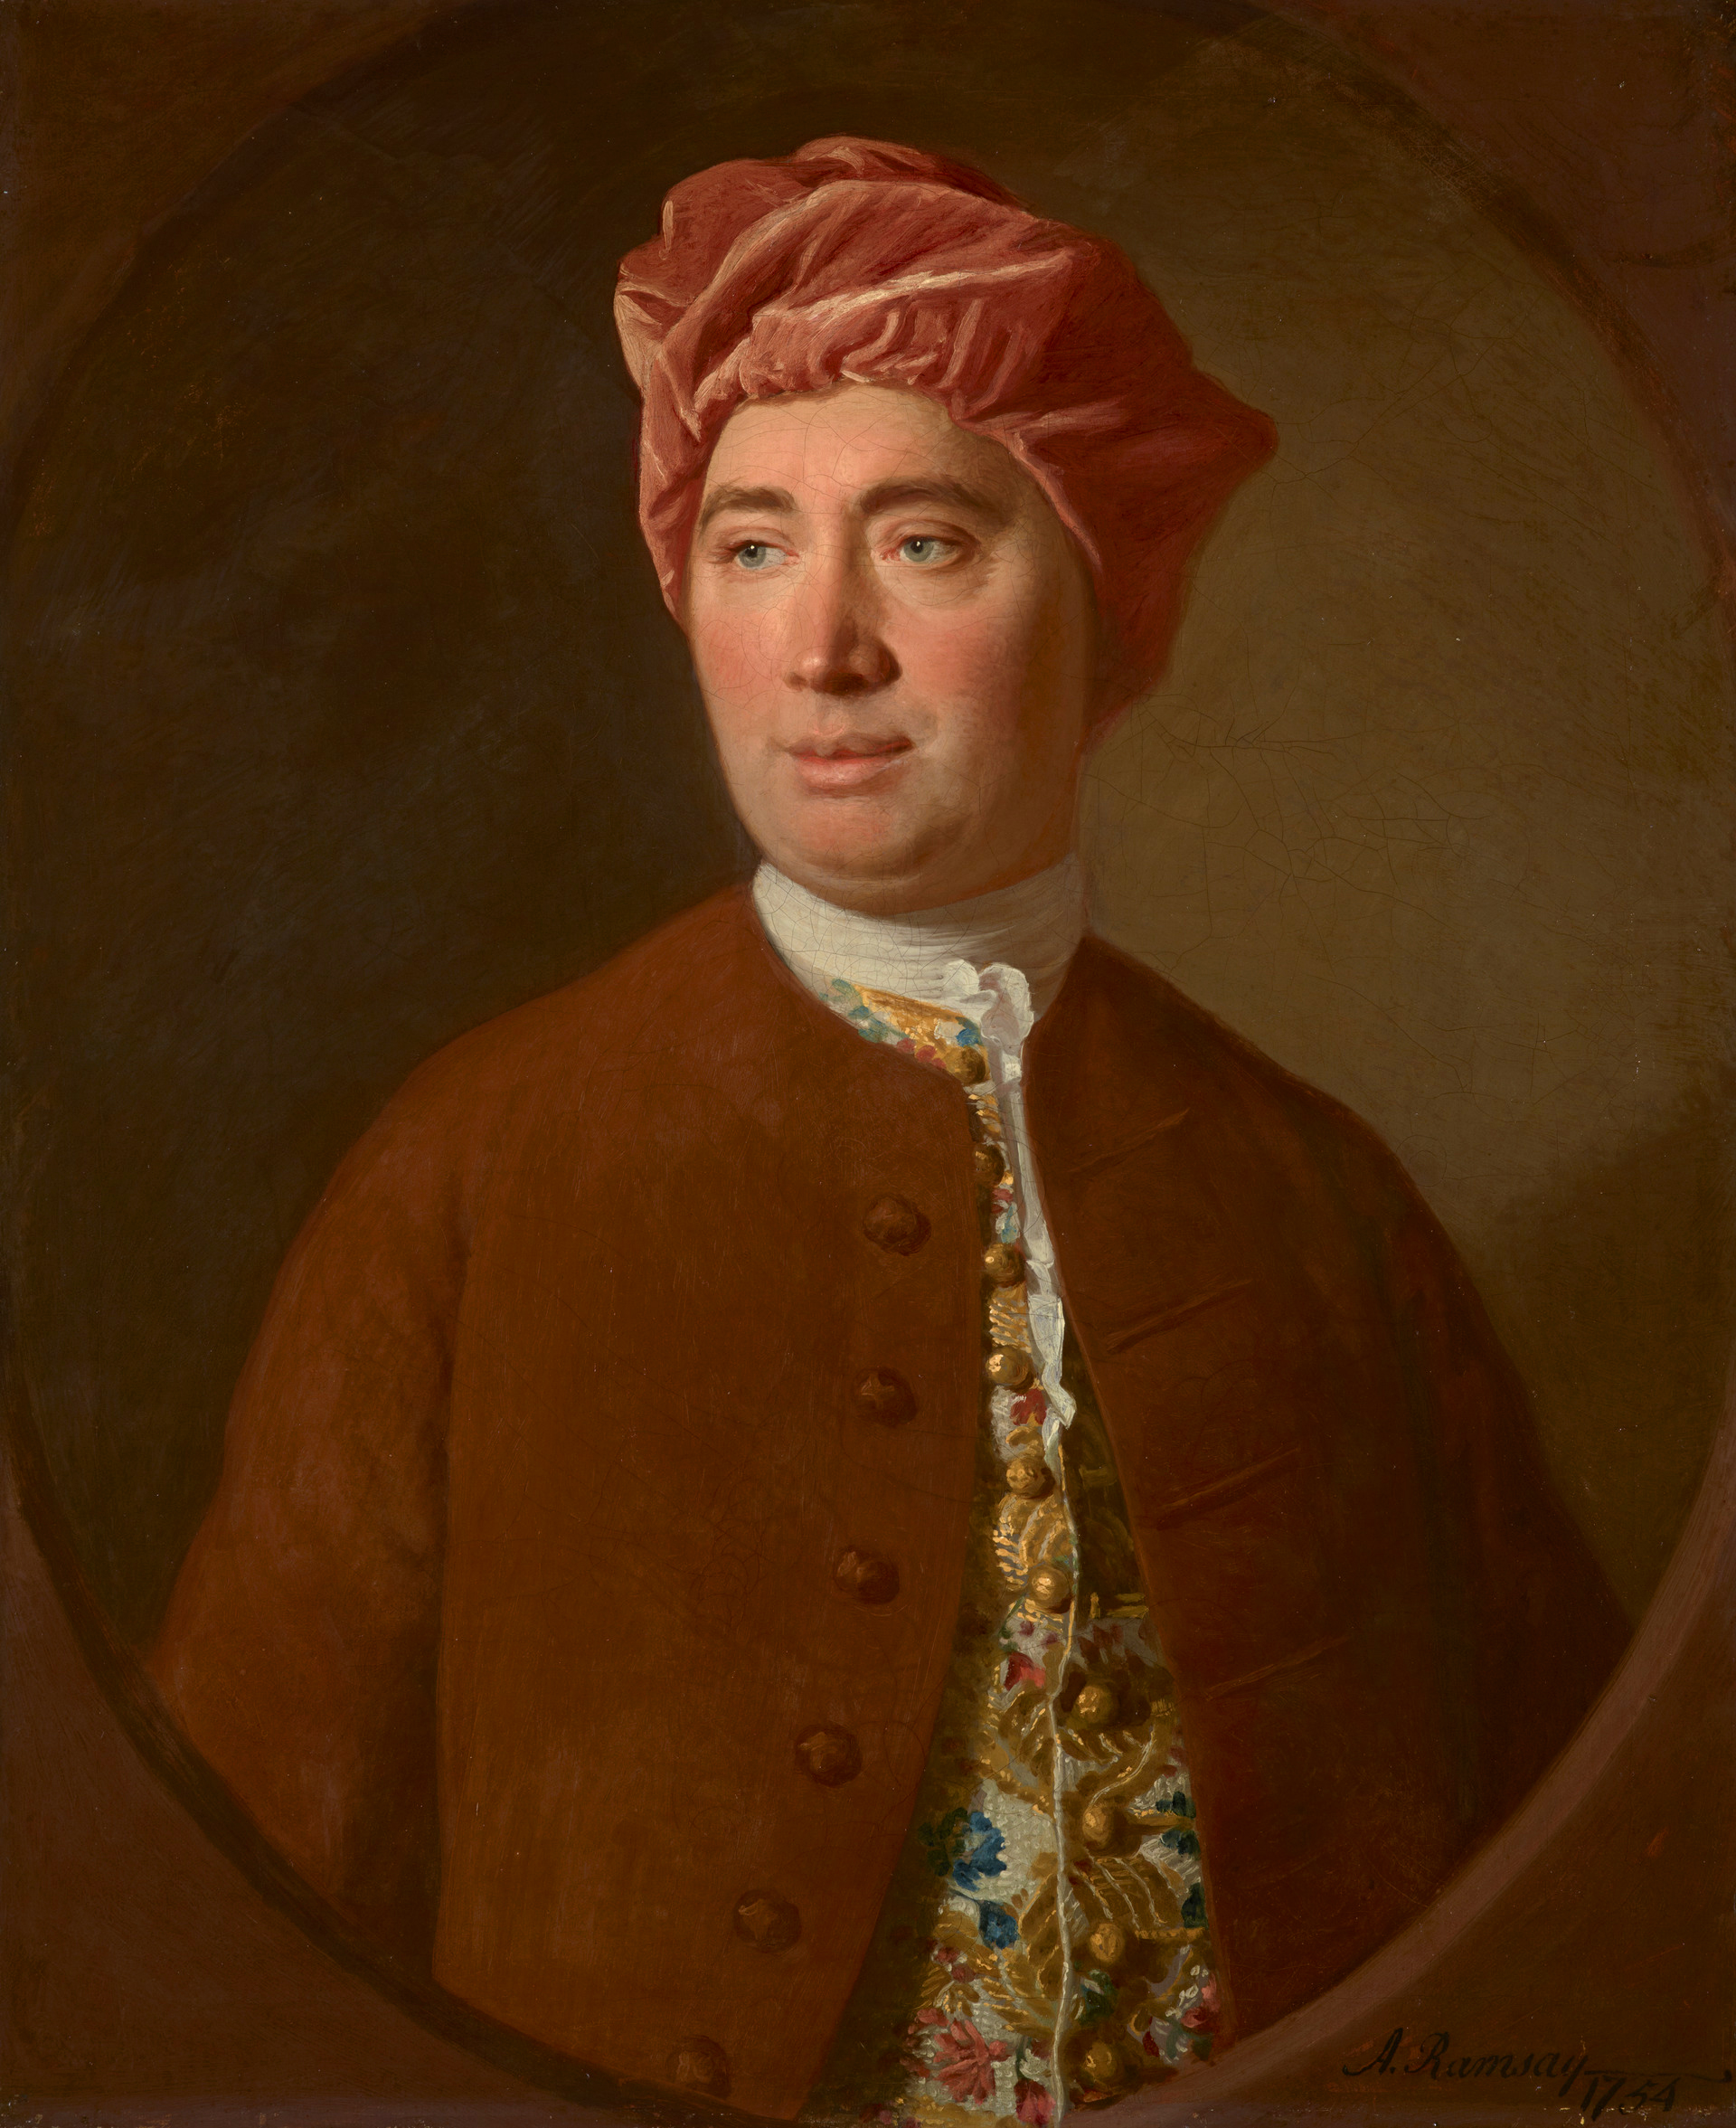
\includegraphics[width=0.26\textwidth]{./figures/aula3_hume.jpg}} \qquad
        \subfloat[\href{https://pt.wikipedia.org/wiki/David_Ricardo}{David Ricardo (1772 - 1823)}]{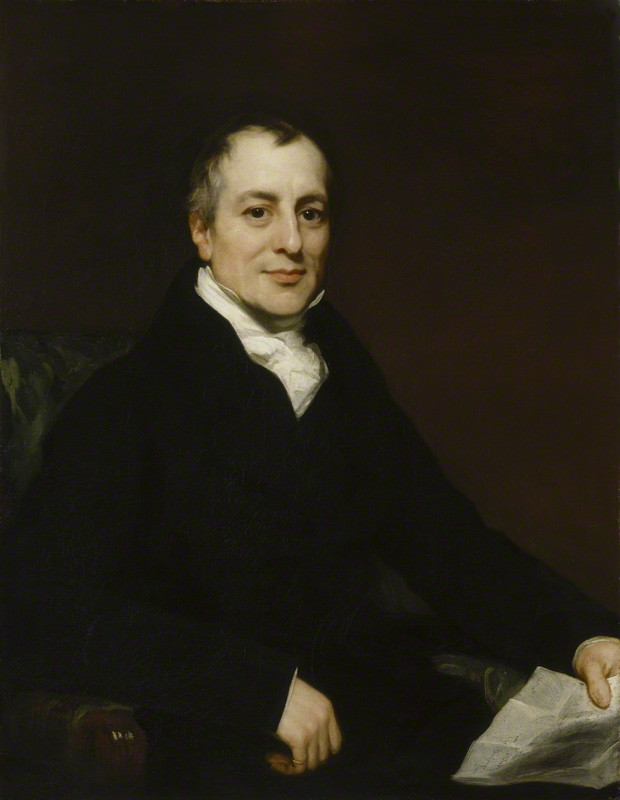
\includegraphics[width=0.25\textwidth]{./figures/aula02_ricardo.jpg}}
        \caption{Economistas que contribuíram para TQM}        
    \end{figure}
\end{frame}

\begin{frame}{Teoria Quantitativa da Moeda}
    \begin{figure}
        \centering
        \subfloat[\href{https://pt.wikipedia.org/wiki/John_Stuart_Mill}{John Stuart Mill (1806 - 1873)}]{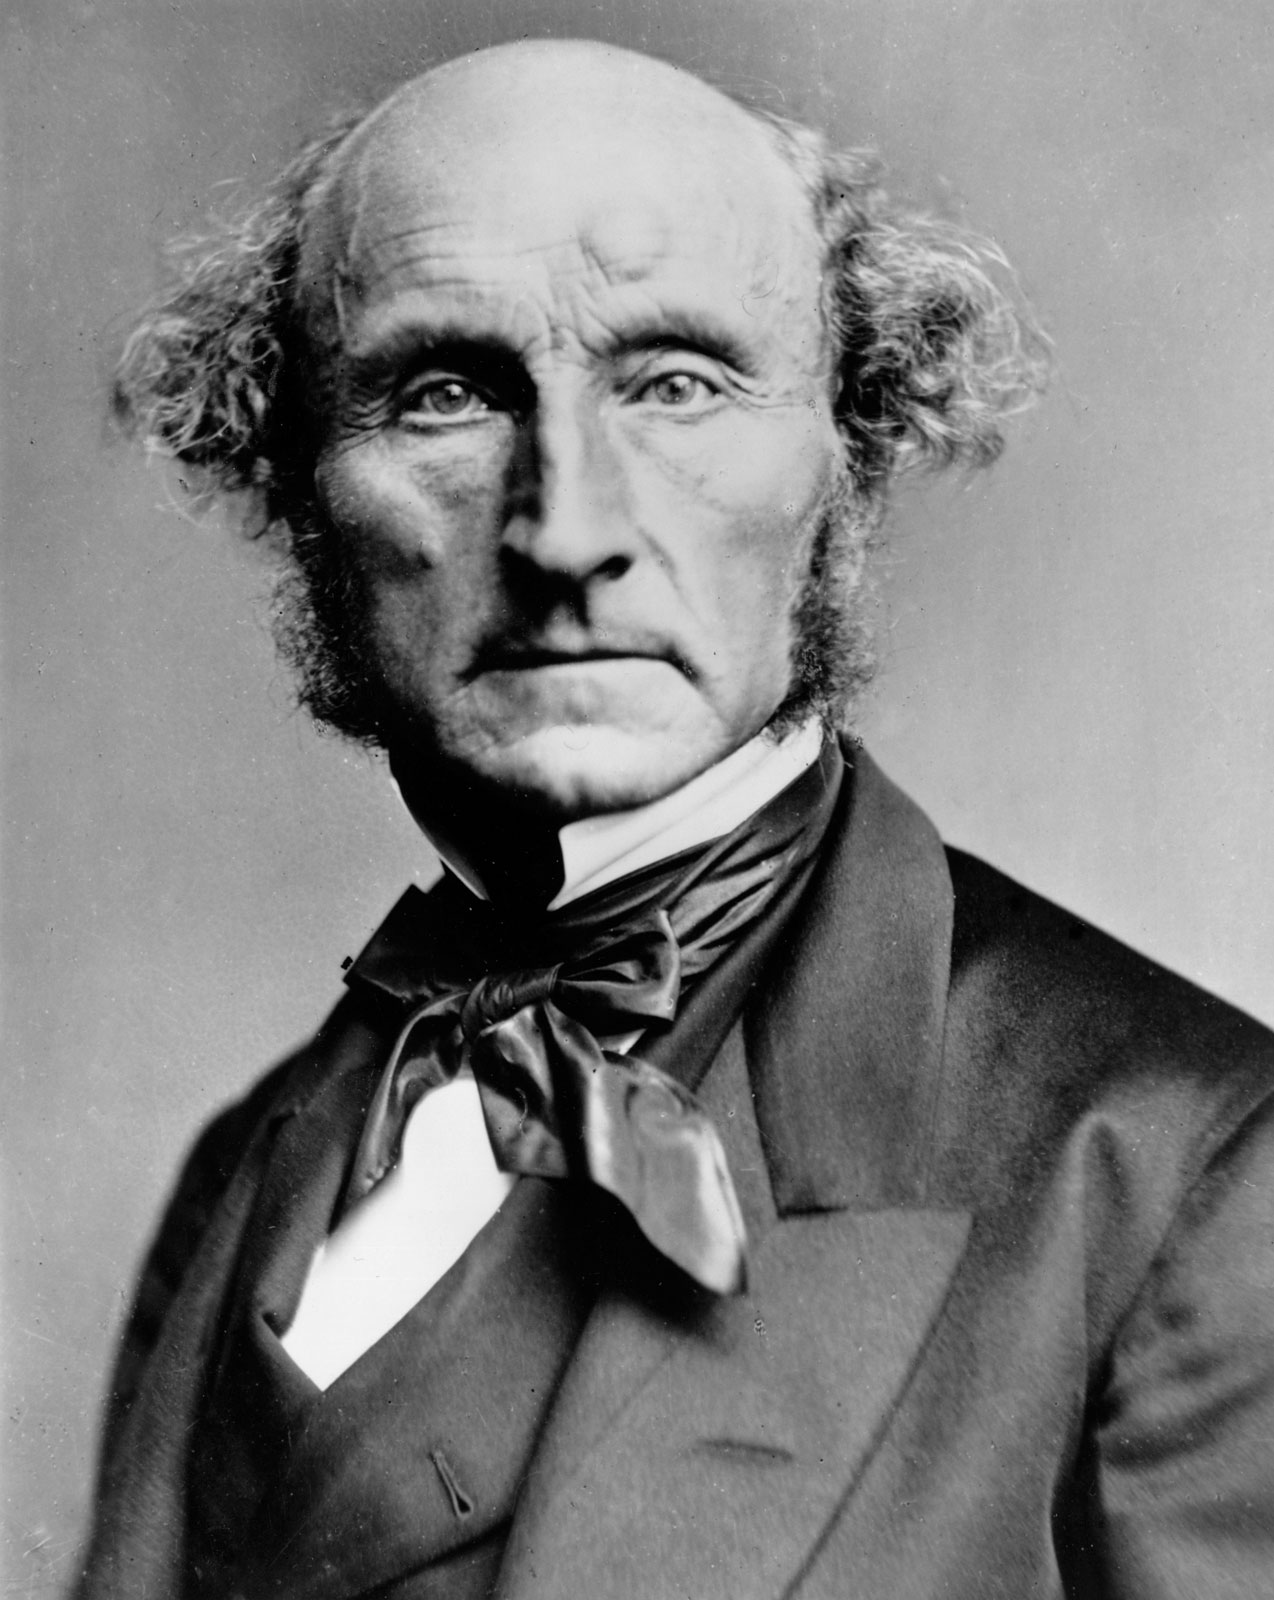
\includegraphics[width=0.3\textwidth]{./figures/aula02_mill.jpg}} \qquad
        \subfloat[\href{https://pt.wikipedia.org/wiki/Alfred_Marshall}{Alfred Marshall (1842 - 1924)}]{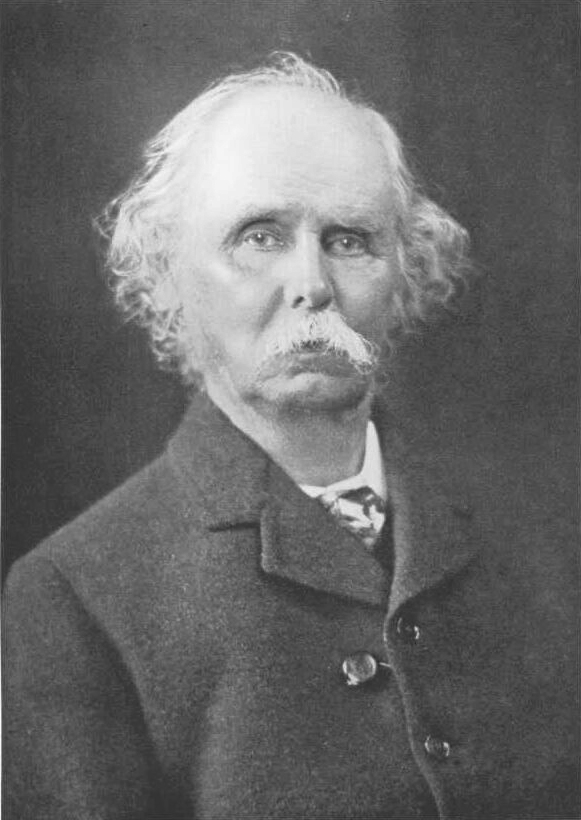
\includegraphics[width=0.26\textwidth]{./figures/aula02_marshall.jpg}} \qquad
        \subfloat[\href{https://pt.wikipedia.org/wiki/Irving_Fisher}{Irving Fisher (1867 - 1947)}]{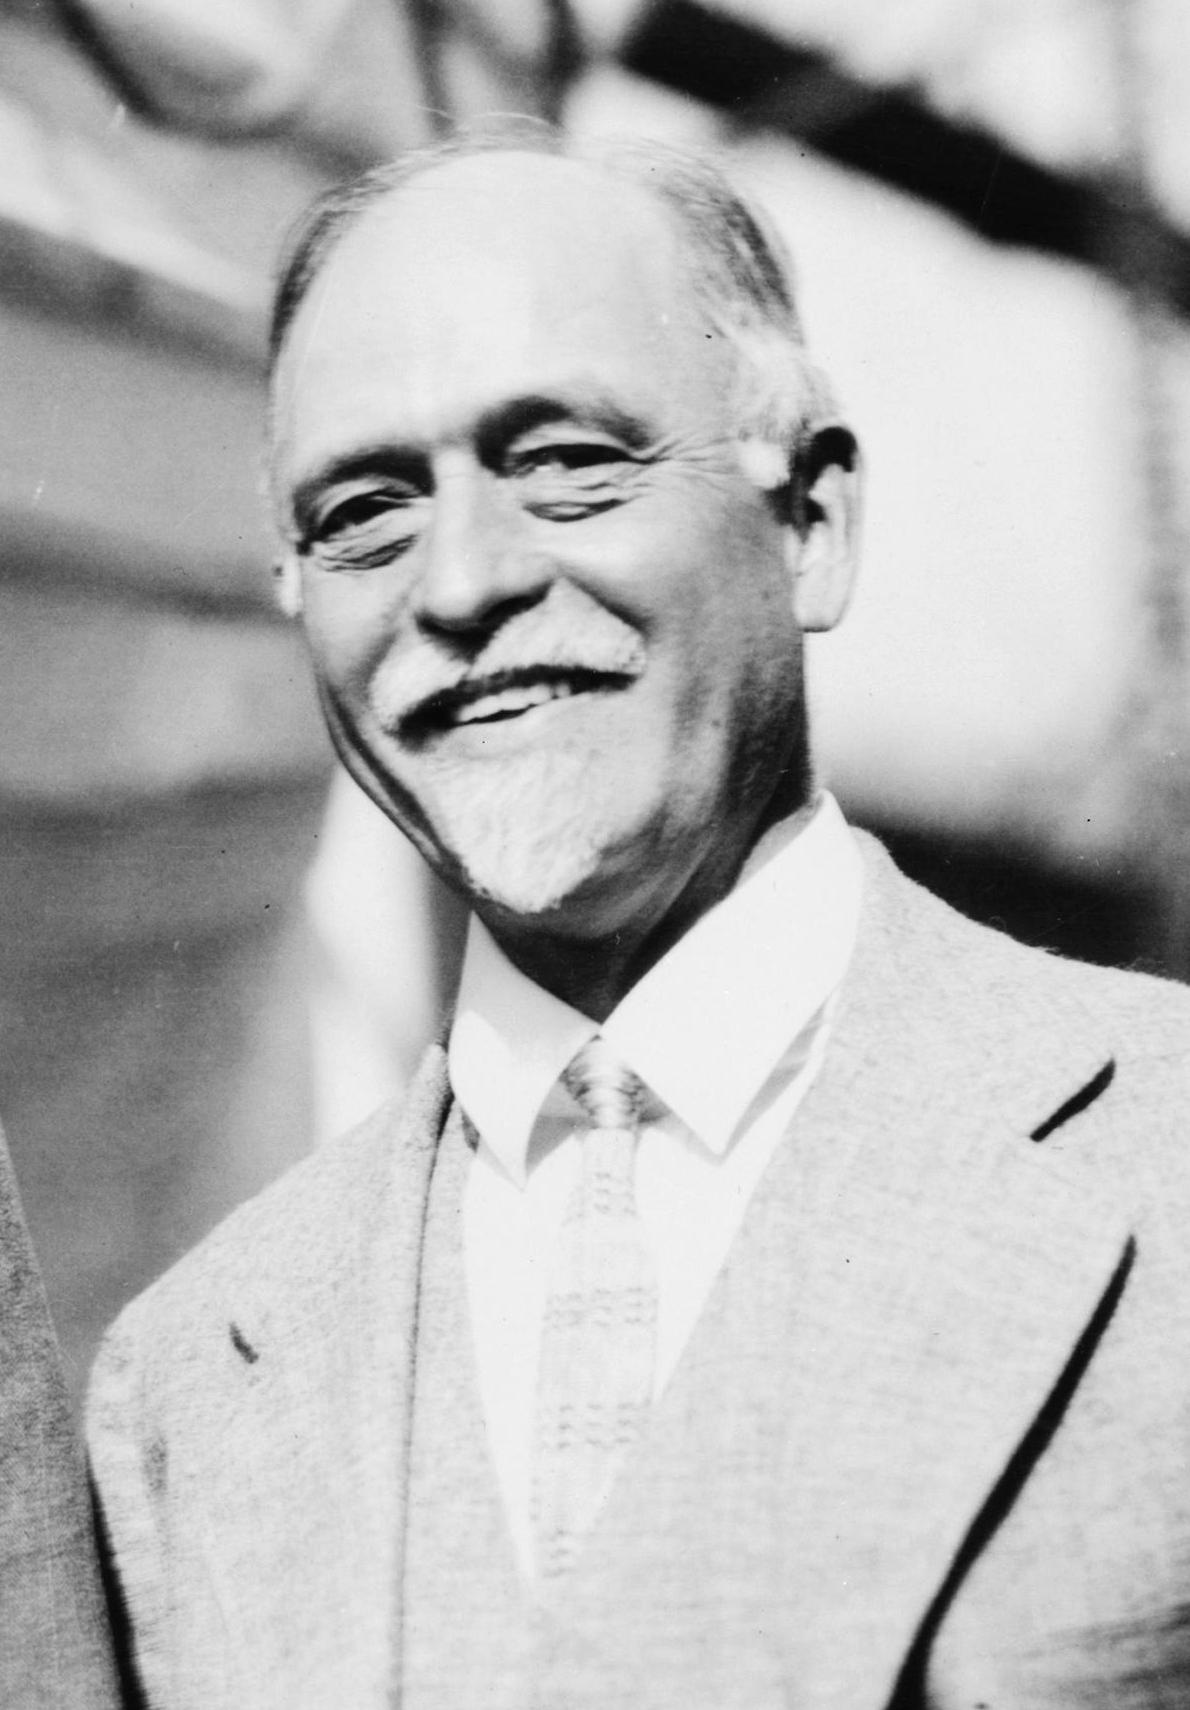
\includegraphics[width=0.25\textwidth]{./figures/aula03_fisher.jpg}}
        \caption{Economistas que contribuíram para TQM}        
    \end{figure}
\end{frame}

\begin{frame}{Teoria Quantitativa da Moeda}
    \begin{figure}
        \centering
        \subfloat[\href{https://pt.wikipedia.org/wiki/Arthur_Cecil_Pigou}{Arthur Cecil Pigou (1877 - 1959)}]{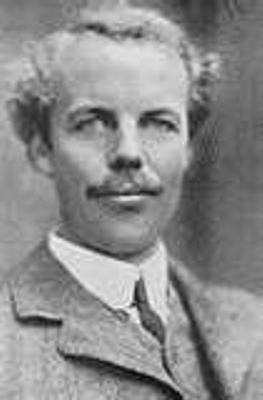
\includegraphics[width=0.2\textwidth]{./figures/aula02_pigou.jpg}} \qquad
        \subfloat[\href{https://pt.wikipedia.org/wiki/Friedrich_Hayek}{Friedrich Hayek (1899 - 1992)}]{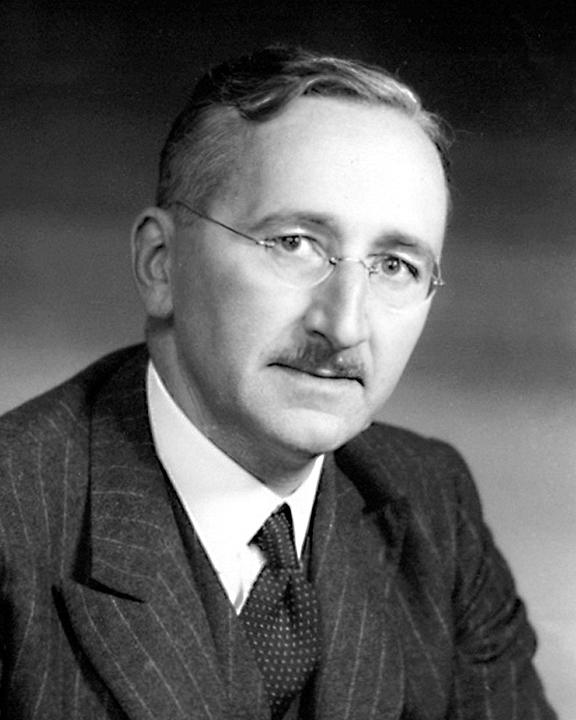
\includegraphics[width=0.25\textwidth]{./figures/aula3_hayek.jpg}} \qquad
        \subfloat[\href{https://pt.wikipedia.org/wiki/John_Maynard_Keynes}{John Maynard Keynes (1883 - 1946)}]{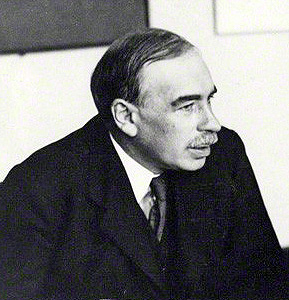
\includegraphics[width=0.3\textwidth]{./figures/aula3_keynes.jpg}}
        \caption{Economistas que contribuíram para TQM}        
    \end{figure}
\end{frame}

\begin{frame}{Teoria Quantitativa da Moeda}
    \begin{tabular}{cl}
        \begin{tabular}{c}
            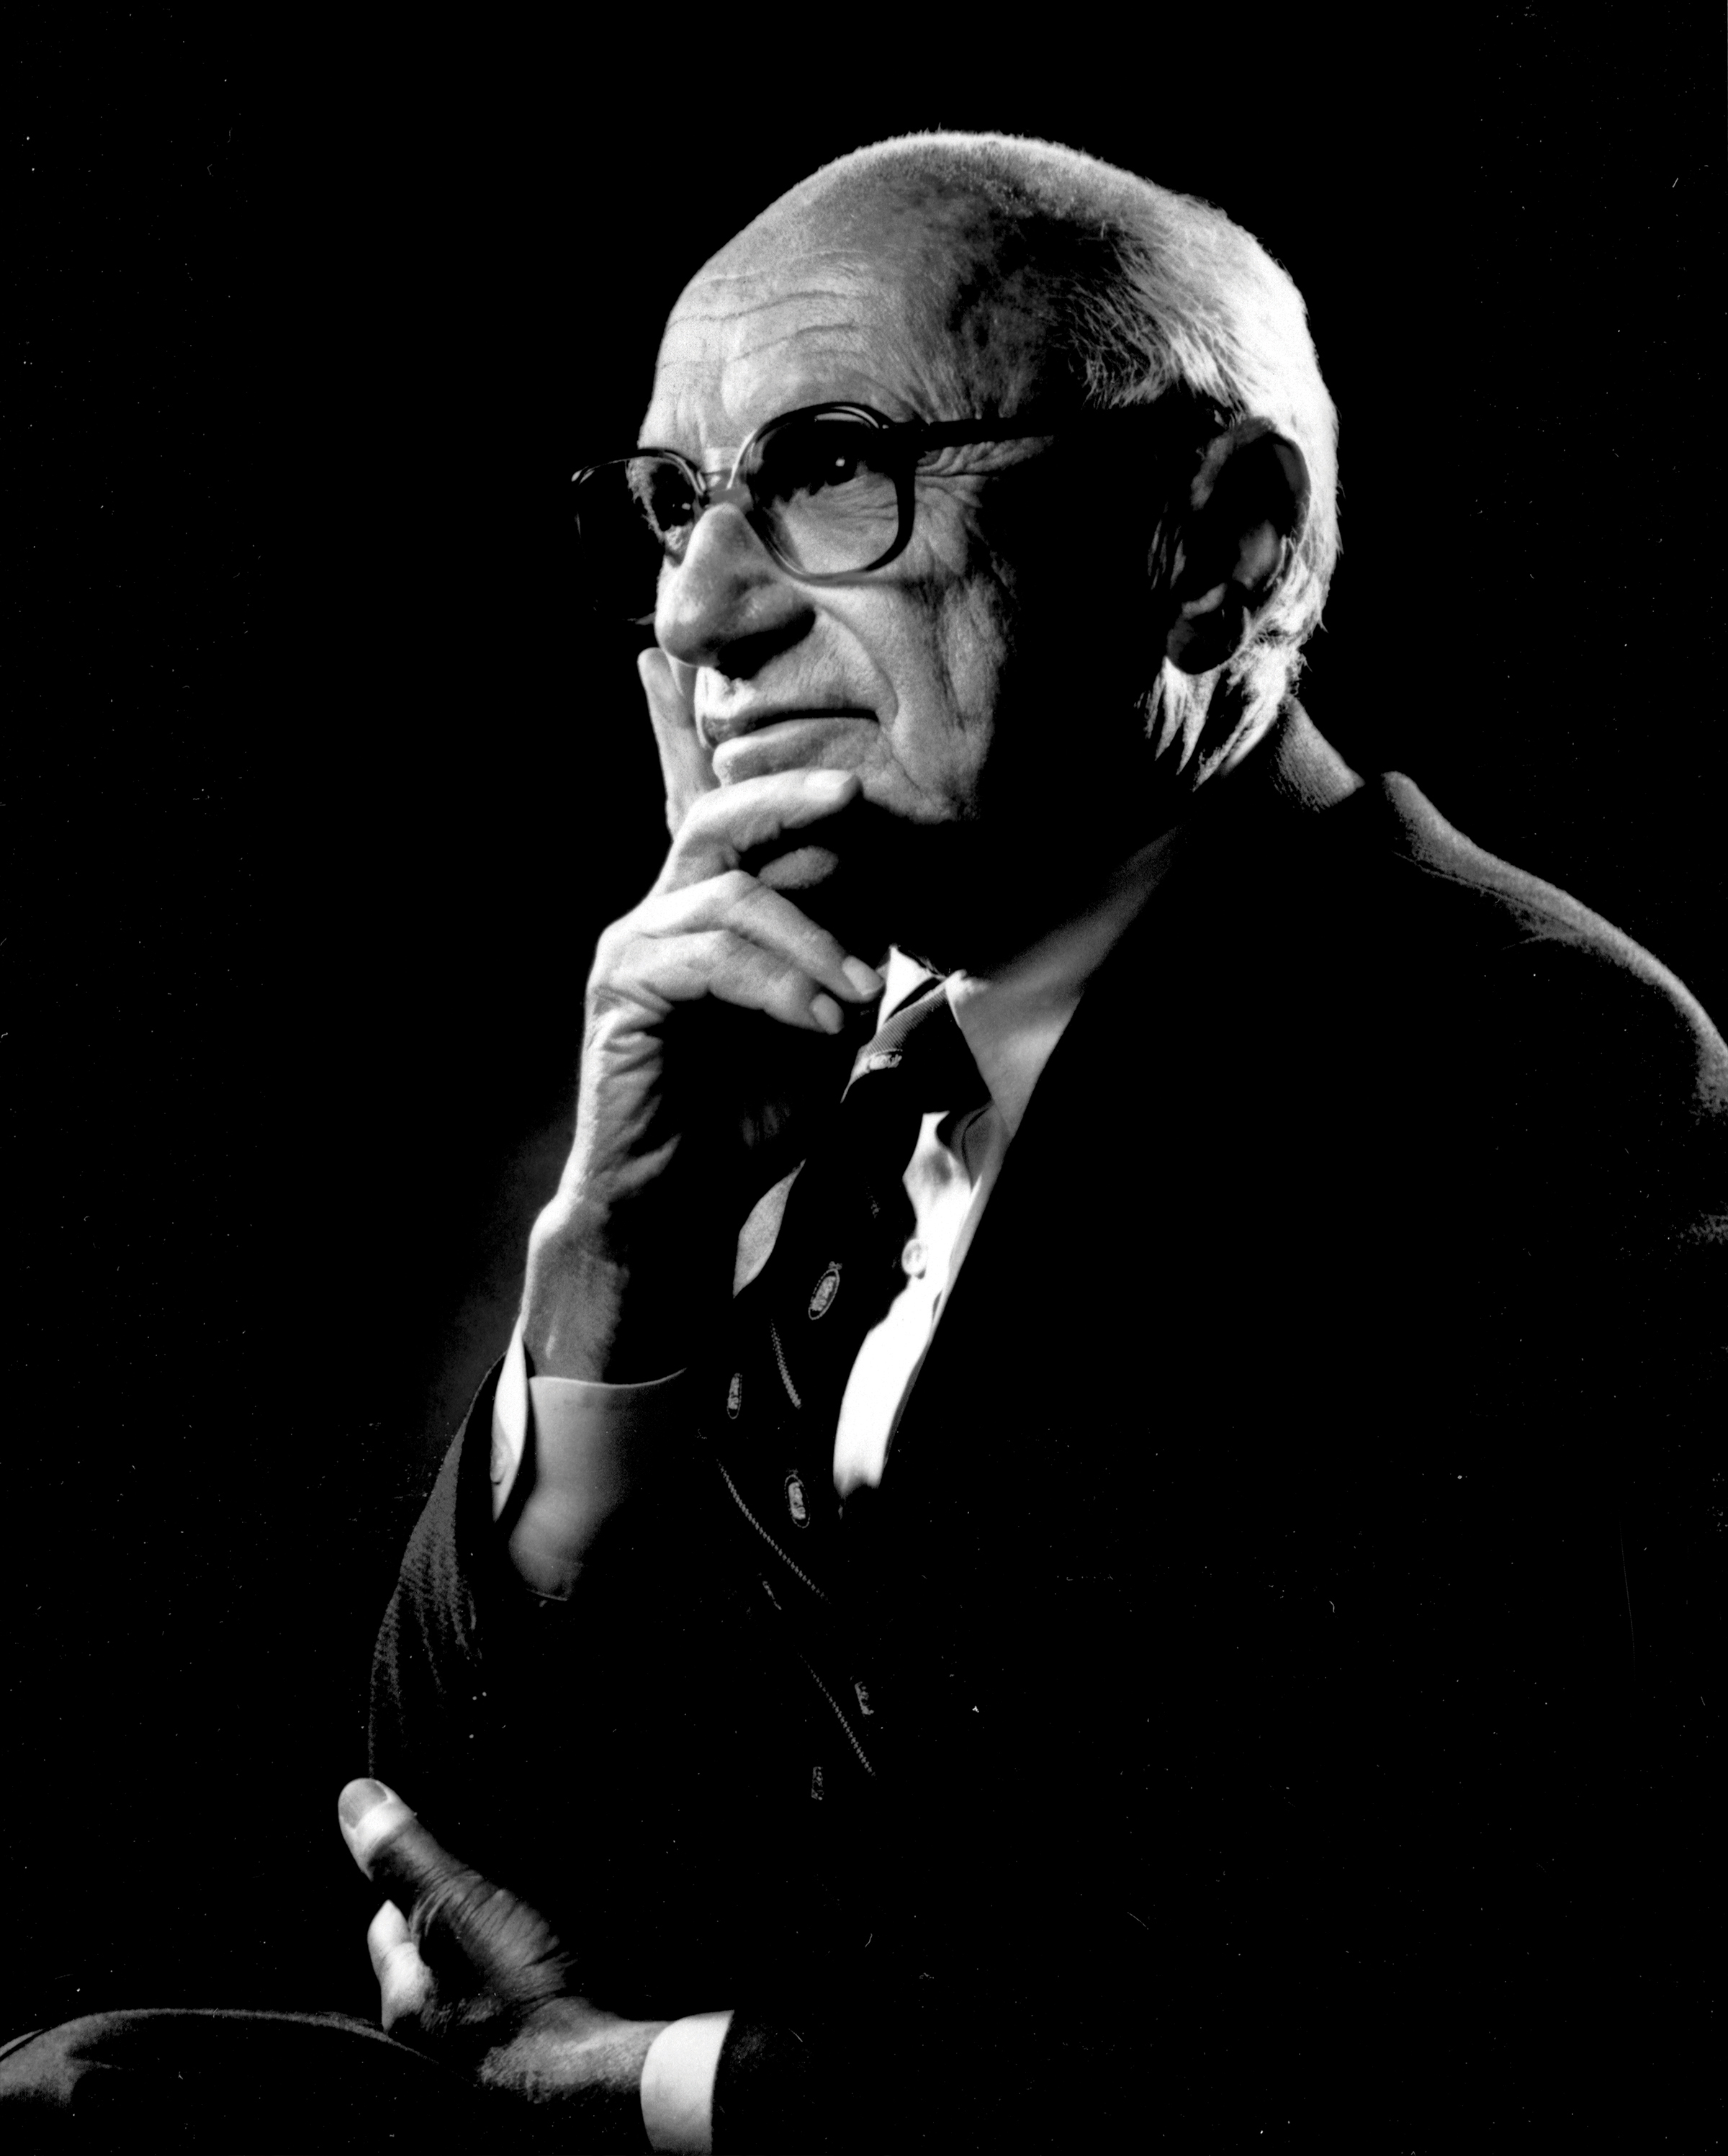
\includegraphics[width=3.5cm]{./figures/aula3_friedman.jpg} \\
            \tiny{{\scshape \href{https://pt.wikipedia.org/wiki/Milton_Friedman}{Milton Friedman (1912 - 2006):}} proponente do monetarismo}
        \end{tabular}
         & \begin{tabular}{l}
               \parbox{0.6\linewidth}{%  change the parbox width as appropiate
                   \begin{itemize}
                    \item Recentemente, TQM associada ao desenvolvimento do monetarismo\bigskip
                    \item Apesar de o termo \hlight{monetarismo} não ter emergido até 1968, sua principal proposição (a TQM) estava bem estabelecida na macro clássica após a publicação de \emph{On Money} - David Hume, 1752\bigskip
                    \item Thomas Mayer, em 1980, argumentou que o nascimento das ideias monetaristas foi em 1752, dado que suas proposições fundamentais já estavam presentes no ensaio de Hume
                   \end{itemize}
               }
           \end{tabular} \\
    \end{tabular}
\end{frame}

\begin{frame}
    {Teoria Quantitativa da Moeda}
    \begin{itemize}
        \item Para entender determinação do nível de preços, analisaremos papel da moeda\bigskip
        \item Modelo clássico: quantidade de moeda em circulação determina demanda agregada que, por sua vez, determina nível de preços\bigskip
        \item Teoria macro dominante pré-1930: TQM\bigskip
        \item Duas versões influentes podem ser identificadas na literatura:\medskip
        \begin{enumerate}
            \item \tikz[tstyle]{\node[nstyle](node0){Abordagem Fisheriana (equação de trocas)}} - associada a Irving Fisher\medskip
            \item \tikz[tstyle]{\node[nstyle](node1){Abordagem de Cambridge}} - associada a Alfred Marshall e Arthur Pigou
        \end{enumerate}                
    \end{itemize}
    \begin{tikzpicture}[tpstyle]
        \draw[pencil,very thick, brick] ([yshift=-1pt]node0.south west) to ([yshift=-1pt]node0.south east);        
        \draw[pencil,very thick, blue] ([yshift=-1pt]node1.south west) to ([yshift=-1pt]node1.south east);
    \end{tikzpicture}
\end{frame}

\begin{frame}
    {Equação de trocas de Fisher}
    \begin{itemize}
        \item A \hlight{equação de trocas} é uma identidade que relaciona o volume de transações a preços correntes à oferta de moeda multiplicada pela taxa de circulação de cada unidade monetária\bigskip
        \item Velocidade de circulação da moeda, que representa o nº médio de vezes que uma unidade monetária é utilizada em transações finais que constituem o PIB nominal - \textcolor{purple}{velocidade da moeda}\bigskip
        \item Equação de trocas de Fisher:
        \begin{equation}
            MV_t \equiv P_t T,
            \label{aula3_eq4}
        \end{equation}
        $M$ quantidade de moeda em circulação, $V_t$ velocidade de transações da moeda, $P_t$ índice de preços dos itens transacionados e $T$ volume de transações
    \end{itemize}
\end{frame}

\begin{frame}
    {Equação de trocas de Fisher}
    \begin{itemize}
        \item Equação (\ref{aula3_eq4}) - identidade devido à definição \emph{ex post} de velocidade\bigskip
        \item Para um dado valor nominal de transações a preços correntes ($P_tT$), a velocidade de circulação da moeda é definida como o nº médio de vezes que a mesma moeda foi usada em transações:
        \[
          V_t \equiv \frac{P_tT}{M}  
        \]
        \item O volume de transações $T$ inclui não só vendas e compras de bens e serviços recém-produzidos mas, também, trocas de ativos financeiros e bens produzidos em períodos anteriores
    \end{itemize}
\end{frame}

\begin{frame}
    {Equação de trocas de Fisher}
    \begin{itemize}
        \item Uma forma alternativa da equação de trocas foca, apenas, nas transações em termos de renda:
        \begin{equation}
            MV \equiv PY,
            \label{aula3_eq5}
        \end{equation}
        $M$ quantidade de moeda em circulação, $P$ índice de preços do produto produzido, $Y$ nível de produção corrente e, agora, $V$ é a velocidade-renda de circulação da moeda, i.e., nº médio de vezes que uma unidade monetária é utilizada em transações finais que constituem PIB nominal
    \end{itemize}
\end{frame}

\begin{frame}
    {Equação de trocas de Fisher}
    \begin{itemize}
        \item A equação de trocas (\ref{aula3_eq5}), que adotaremos, é um truísmo e não explica as variáveis que contém\bigskip
        \item Mas Fisher argumenta que os valores de equilíbrio de seus componentes são exógenas ao modelo. Portanto, a equação de trocas determina o nível de preços\bigskip
        \item Produto agregado - medida da atividade econômica real (determinada por fatores de oferta)\bigskip
        \item Quantidade de moeda em circulação - determinada exogenamente pela autoridade monetária\bigskip
        \item Nível de equilíbrio da velocidade de circulação da moeda - determinada por fatores institucionais (hábitos e tecnologia de pagamentos da sociedade) pode ser tomada como constante no curto prazo
    \end{itemize}
\end{frame}

\begin{frame}
    {Equação de trocas de Fisher}
    \begin{itemize}
        \item Se $V$ é predeterminada e não definida residualmente (para igualar $MV$ e $PY$), a equação de trocas não é meramente uma definição\bigskip
        \item Com o produto determinado pelo lado da oferta, a equação de trocas Fisheriana expressa uma relação de proporcionalidade entre oferta de moeda e nível de preços:
        \begin{equation}
            P = \frac{\bar{V}}{\bar{Y}}M
            \label{aula3_eq6}
        \end{equation}
        \item Temos, então, o resultado fundamental da TQM\bigskip
        \item \hlight{A quantidade de moeda em circulação, $M$, determina o nível de preços, $P$}\bigskip
        \item Além disso, $\Delta M = \Delta P$
    \end{itemize}
\end{frame}

\begin{frame}
    {Abordagem de Cambridge}
    \begin{itemize}
        \item Versão Fisheriana: clara mas mecanicista\bigskip
        \item Qual a intuição econômica para entendermos como mudanças na oferta monetária afetam nível de preços?\bigskip
        \item \hlight{Abordagem de Cambridge}: também apresenta relação proporcional entre qtdade de moeda em circulação e nível agregado de preços\bigskip
        \item Mas esboçam uma distinção clara, em sua versão da TQM, entre demanda por moeda ($M^d$) e oferta monetária ($M$)
    \end{itemize}
\end{frame}

\begin{frame}
    {Abordagem de Cambridge}
    \begin{itemize}
        \item Abordagem de Cambridge - foco nas decisões individuais de quantidade ótima de moeda a ser retida\bigskip
        \item Por que indivíduos optam por reter moeda?\bigskip
        \item Demanda por moeda é determinada, principalmente, pela necessidade de realizar transações (o que terá uma relação positiva com o valor nominal de gastos agregados)\bigskip
        \item A moeda mantida em poder dos indivíduos não gera renda\bigskip
        \item Portanto, só será mantida na medida em que suas vantagens em termos de motivo transação superem a renda perdida por não investir em atividades produtivas, aquisição de bens de consumo ou ativos que rendam juros
    \end{itemize}
\end{frame}

\begin{frame}
    {Abordagem de Cambridge}
    \begin{itemize}
        \item Qual a quantidade ótima de moeda a ser mantida?\bigskip
        \item Abordagem de Cambridge assume que a demanda por moeda ($M^d$) seria uma proporção $k$ da renda nominal ($PY$):
        \begin{equation}
            M^d = kPY
            \label{aula3_eq7}
        \end{equation}
        \item A característica desejável da moeda é sua utilidade para transações\bigskip
        \item Portanto, demanda por moeda depende positivamente do nível de transações na economia que, pode-se supor, varie positivamente com a renda
    \end{itemize}
\end{frame}

\begin{frame}
    {Abordagem de Cambridge}
    \begin{itemize}
        \item Proporção ótima da renda a ser mantida sob forma de moeda, $k$, é considerada estável no curto prazo (depende dos hábitos de pagamento da sociedade)\bigskip
        \item Para explicar nível de preços, devemos introduzir oferta de moeda\bigskip
        \item Se oferta de moeda é determinada exogenamente pela autoridade monetária, temos a condição de equilíbrio:
        \begin{equation}
            M = M^d = kPY
            \label{aula3_eq8}
        \end{equation}
        \item $k$ fixo no curto prazo + produto real determinado por condições de oferta = equação de Cambridge também se reduz a uma relação proporcional entre nível de preços e oferta de moeda
    \end{itemize}
\end{frame}

\begin{frame}
    {Equivalência formal entre abordagens}
    \begin{itemize}
        \item Reescrevendo equação (\ref{aula3_eq8}) podemos notar equivalência formal entre abordagens:
        \[
          M\frac{1}{k} = P\bar{Y}  
        \]
        \item Portanto, a velocidade de circulação da moeda $V$ é o recíproco da proporção de moeda que os indivíduos decidem manter, $k$\bigskip
        \item E.g., se indivíduos optam por manter 1/4 da renda nominal em forma de moeda, o nº médio de vezes que a moeda é usada em transações de renda será igual a 4\bigskip
        \item Equivalência formal entre as duas versões, mas versão de Cambridge é um passo na direção de teorias monetárias modernas (teoria de demanda por moeda)\bigskip
        \item Seguindo abordagem de Pigou e Marshall, Keynes contrapôs-se à TQM com uma nova teoria de demanda por moeda
    \end{itemize}
\end{frame}

\section{Determinação de variáveis nominais}

\begin{frame}
    {Determinação de variáveis nominais}
    \begin{itemize}
        \item Como o nível de preços é determinado no modelo clássico?\bigskip
        \item Como produto real, salários reais e nível de emprego são invariantes a mudanças na quantidade de moeda em circulação?
    \end{itemize}
\end{frame}

\begin{frame}
    \begin{figure}
        \centering
        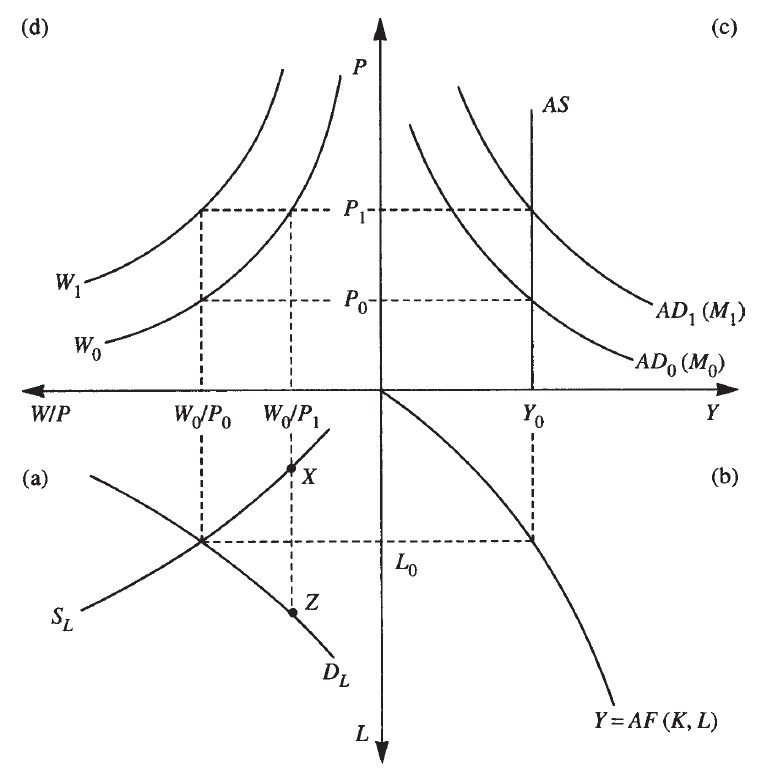
\includegraphics[width=0.5\textwidth]{./figures/aula3_fig3.PNG}
        \caption{Determinação do nível de preços. Fonte: Snowdon e Vane (2005).}
        \label{aula3_fig3}
    \end{figure}
\end{frame}

\begin{frame}
    {Determinação de variáveis nominais}
    \begin{itemize}
        \item Paineis (a) e (b) - determinação do nível de emprego e produto agregados\bigskip
        \item Mercado de trabalho perfeitamente competitivo gera um nível de emprego de equilíbrio $L_0$ e salário real $W_0/P_0$\bigskip
        \item Pela função de produção agregada, $L_0$ corresponde a um produto de pleno emprego $Y_0$ (assumindo versão forte da Lei de Say)\bigskip
        \item Painel (c) - curvas clássicas de demanda agregada (AD) e oferta agregada (AS)\bigskip
        \item Curva de oferta agregada clássica é perfeitamente inelástica (vertical) - produto real invariante a alterações no nível geral de preços
    \end{itemize}    
\end{frame}

\begin{frame}
    {Determinação de variáveis nominais}
    \begin{itemize}
        \item Curva de demanda agregada clássica - derivada da equação de trocas $MV = PY$\bigskip
        \item Oferta de moeda constante + velocidade de circulação da moeda fixa no curto prazo - nível de preços mais alto deve estar associado a nível de produto real mais baixo (AD negativamente inclinada)\bigskip
        \item $AD_0(M_0)$ mostra que, dada oferta monetária, temos infinitas combinações de $P$ e $Y$ que dão resultado igual a $MV$\bigskip
        \item Como assumimos $V$ fixo, o valor nominal de todas as transações é determinado pela oferta de moeda\bigskip
        \item A níveis de preços mais elevados, cada transação requer um nº maior de unidades monetárias e, portanto, a qtdade. de bens e serviços que podem ser adquiridos deve cair (para uma oferta de moeda fixa)\bigskip
        \item Por fim, um aumento na oferta de moeda desloca $AD$ para a direita - $AD_1(M_1)$
    \end{itemize}
\end{frame}

\begin{frame}
    {Determinação de variáveis nominais}
    \begin{itemize}
        \item Painel (d) - relação entre salário real e nível geral de preços para um dado nível de salário nominal\bigskip
        \item Se o salário nominal é igual a $W_0$, um aumento do nível de preços reduz o salário real\bigskip
        \item Deslocamento ao longo da curva $W_0$ de $(W_0/P_0, P_0)$ para $(W_0/P_1, P_1)$
    \end{itemize}
\end{frame}

\begin{frame}
    {Política monetária}
    \begin{itemize}
        \item Assuma que os valores iniciais de equilíbrio associados a $M_0$ sejam $Y_0, W_0/P_0$ e $L_0$\bigskip
        \item Suponha que a autoridade monetária aumente oferta monetária para $M_1$ numa tentativa de estimular produto real e nível de emprego\bigskip
        \item Aumento na qtdade de moeda em circulação cria desequilíbrio no mercado monetário - excesso de oferta de moeda $M^d<M$\bigskip
        \item Portanto, temos um aumento na demanda por bens e serviços\bigskip
        \item Com produto real $Y_0$ fixado pelas condições de equilíbrio no mercado de trabalho perfeitamente competitivo a um nível de emprego $L_0$, o nível de preços aumenta de $P_0$ para $P_1$
    \end{itemize}
\end{frame}

\begin{frame}
    {Política monetária}
    \begin{itemize}
        \item Para um dado salário nominal $W_0$, o aumento no nível de preços reduz o salário real e, portanto, causa desequilíbrio no mercado de trabalho\bigskip
        \item Excesso de demanda por trabalho de magnitude $ZX$ emerge a um salário real $W_0/P_1$\bigskip
        \item O excesso de demanda por trabalho leva trabalhadores a barganharem um nível salarial mais alto\bigskip
        \item Salário nominal se eleva até o valor $W_1$, restaurando salário real ao nível de equilíbrio $W_0/P_0 = W_1/P_1$
    \end{itemize}
\end{frame}

\begin{frame}
    {Política monetária}
    \begin{itemize}
        \item Por fim, a expansão monetária aumenta taxa de juros nominal via \hlight{efeito Fisher}\bigskip
        \item No modelo clássico, taxa de juros real se ajusta para equalizar poupança e investimento no mercado de fundos emprestáveis\bigskip
        \item Pela equação de Fisher, a taxa real de juros ($r$) é igual à taxa nominal ($i$) menos a taxa de inflação ($\pi$):
        \begin{equation}
            r = i - \pi
            \label{aula3_eq9}
        \end{equation}
        \item Vimos que a taxa de juros real é determinada pelas forças reais de produtividade e parcimônia\bigskip
        \item Portanto, a taxa de juros nominal se ajusta para refletir as variações tanto da taxa real de juros quanto da taxa de inflação\bigskip
        \item A expansão monetária, ao aumentar a taxa de inflação, leva a um aumento proporcional da taxa nominal de juros
    \end{itemize}
\end{frame}

\begin{frame}
    {Política monetária}
    \begin{itemize}
        \item Em resumo, \textcolor{blue}{uma política monetária expansionista leva a aumento do nível geral de preços, salários nominais e taxa nominal de juros, enquanto variáveis agregadas reais permanecem inalteradas} - \hlight{neutralidade da moeda}\bigskip
        \item Essa relação direta entre expansão monetária e aumento generalizado do nível de preços é observado claramente em períodos de hiperinflação\bigskip
        \item Alemanha agosto/1922 - novembro/1923: taxa mensal de inflação de 322\% e taxa de crescimento da base monetária de 314\%\bigskip
        \item Hungria agosto/1945 - julho/1946: taxa mensal de inflação de 19800\% e taxa de crescimento da moeda de 12200\%
    \end{itemize}
\end{frame}

\begin{frame}
    {Política monetária}
    \begin{figure}
        \centering
        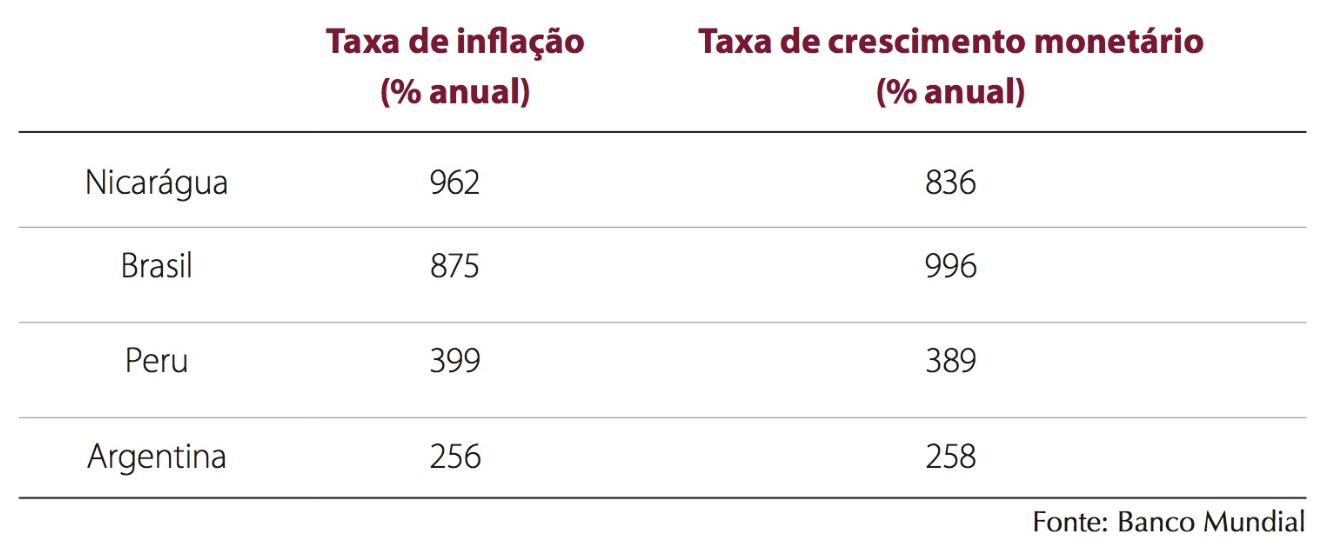
\includegraphics[width=\textwidth]{./figures/aula3_fig4.PNG}
        \caption{Inflação e expansão monetária em economias com alta inflação (1985-1995). Fonte: Froyen (2013).}
        \label{aula3_fig4}
    \end{figure}
\end{frame}

\section{Evidências empíricas}
\begin{frame}
    {Evidências de rigidez nominal}
    \begin{itemize}
        \item \hlight{Evidências sobre rigidez nominal}: a maioria das tentativas de extrair evidências acerca da existência e importância de rigidez de preços usa análise de microdados (dados de preços de bens e serviços individuais)\medskip
        \begin{enumerate}
            \item Taylor(1999) - firmas americanas ajustam preços apenas anualmente (rigidez de preços) e de forma dessincronizada (preços escalonados)\medskip
            \item Dhyne et al. (2006) - resultados similares para área do Euro\medskip
            \item Moura e Rossi Jr. (2010) - resultados similares para Brasil\medskip
            \item Estes estudos apontam, também, para heterogeneidade na duração dos preços (serviços - maior grau de rigidez, alimentos não-processados e energia - menor grau)
        \end{enumerate}
    \end{itemize}
\end{frame}

\begin{frame}
    {Evidências de não-neutralidade da moeda}
    \begin{itemize}
        \item \hlight{Evidências sobre efeitos da política monetária}\bigskip
        \begin{enumerate}
            \item Teoricamente, rigidez de preços implica não-neutralidade da moeda\bigskip
            \item Empiricamente, choques monetários geram\medskip
            \begin{enumerate}
                \item efeitos consideráveis e persistentes de curto prazo no produto\medskip
                \item efeitos apenas tardios no nível de preços - evidência de rigidez nominal\medskip
                \item declínio de M2 (i.e., autoridade monetária deve reduzir qtdade de moeda em circulação para alcançar um aumento da taxa nominal), sugerindo a existência de \hlight{efeito liquidez} (co-movimento negativo entre oferta de moeda e taxa nominal de juros)
            \end{enumerate}
        \end{enumerate}
    \end{itemize}
\end{frame}

\begin{frame}
    {Evidências sobre efeitos da política monetária}
    \begin{figure}
        \centering
        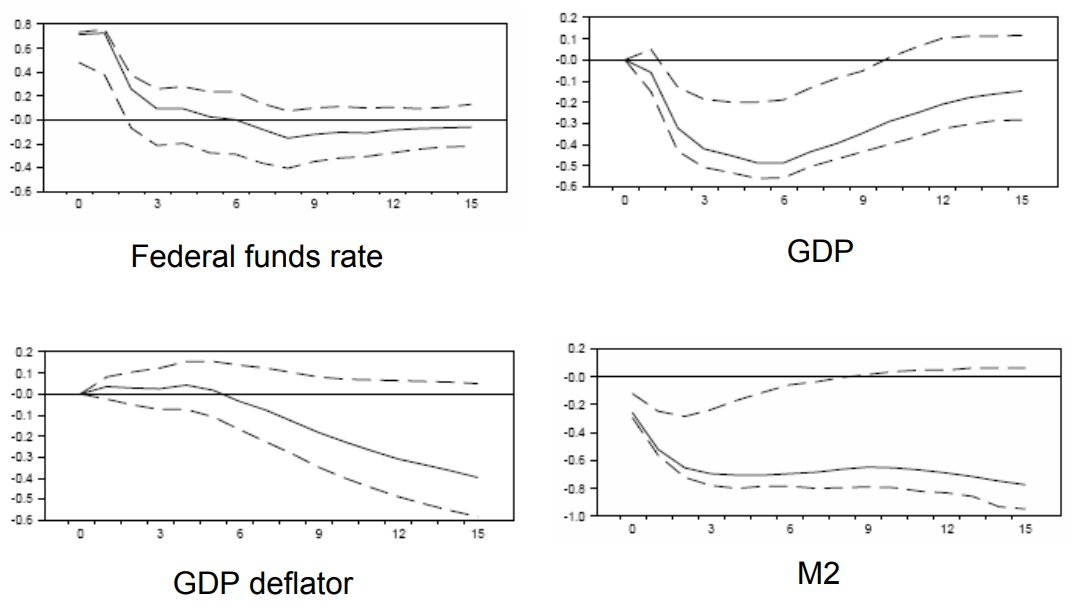
\includegraphics[width=0.7\textwidth]{./figures/aula3_fig5.jpg}
        \caption{Respostas diâmicas estimadas a um choque de política monetária - EUA. Fonte: Christiano, Eichenbaum e Evans (1999).}
        \label{aula3_fig5}
    \end{figure}
\end{frame}

\begin{frame}{\emoji{books} Bibliografia}
    \begin{itemize}
        \item FROYEN, R. \emph{Macroeconomia: teorias e aplicações}. 2.ed. São Paulo: Saraiva, 2013. Disponível em: \href{https://app.minhabiblioteca.com.br/books/9788502175235}{app.minhabiblioteca.com.br/books/9788502175235}\medskip
        \item KEYNES, J.M. \emph{A teoria geral do emprego, do juro e da moeda}. São Paulo: Atlas, 1992. (Data do original em inglês: 1936).\medskip
        \item LOPES, L.M.; VASCONCELLOS, M.A.S. \emph{Manual de Macroeconomia: Nível básico e nível intermediário}. 3.ed. São Paulo: Atlas, 2008.\medskip
        \item SNOWDON, B.; VANE, H.R. \emph{Modern Macroeconomics: its Origins, Development and Current State}. Northampton, MA: Edward Elgar, 2005.
    \end{itemize}
\end{frame}
\end{document}